% Options for packages loaded elsewhere
\PassOptionsToPackage{unicode}{hyperref}
\PassOptionsToPackage{hyphens}{url}
%
\documentclass[
]{book}
\usepackage{amsmath,amssymb}
\usepackage{lmodern}
\usepackage{iftex}
\ifPDFTeX
  \usepackage[T1]{fontenc}
  \usepackage[utf8]{inputenc}
  \usepackage{textcomp} % provide euro and other symbols
\else % if luatex or xetex
  \usepackage{unicode-math}
  \defaultfontfeatures{Scale=MatchLowercase}
  \defaultfontfeatures[\rmfamily]{Ligatures=TeX,Scale=1}
\fi
% Use upquote if available, for straight quotes in verbatim environments
\IfFileExists{upquote.sty}{\usepackage{upquote}}{}
\IfFileExists{microtype.sty}{% use microtype if available
  \usepackage[]{microtype}
  \UseMicrotypeSet[protrusion]{basicmath} % disable protrusion for tt fonts
}{}
\makeatletter
\@ifundefined{KOMAClassName}{% if non-KOMA class
  \IfFileExists{parskip.sty}{%
    \usepackage{parskip}
  }{% else
    \setlength{\parindent}{0pt}
    \setlength{\parskip}{6pt plus 2pt minus 1pt}}
}{% if KOMA class
  \KOMAoptions{parskip=half}}
\makeatother
\usepackage{xcolor}
\usepackage{color}
\usepackage{fancyvrb}
\newcommand{\VerbBar}{|}
\newcommand{\VERB}{\Verb[commandchars=\\\{\}]}
\DefineVerbatimEnvironment{Highlighting}{Verbatim}{commandchars=\\\{\}}
% Add ',fontsize=\small' for more characters per line
\usepackage{framed}
\definecolor{shadecolor}{RGB}{248,248,248}
\newenvironment{Shaded}{\begin{snugshade}}{\end{snugshade}}
\newcommand{\AlertTok}[1]{\textcolor[rgb]{0.94,0.16,0.16}{#1}}
\newcommand{\AnnotationTok}[1]{\textcolor[rgb]{0.56,0.35,0.01}{\textbf{\textit{#1}}}}
\newcommand{\AttributeTok}[1]{\textcolor[rgb]{0.77,0.63,0.00}{#1}}
\newcommand{\BaseNTok}[1]{\textcolor[rgb]{0.00,0.00,0.81}{#1}}
\newcommand{\BuiltInTok}[1]{#1}
\newcommand{\CharTok}[1]{\textcolor[rgb]{0.31,0.60,0.02}{#1}}
\newcommand{\CommentTok}[1]{\textcolor[rgb]{0.56,0.35,0.01}{\textit{#1}}}
\newcommand{\CommentVarTok}[1]{\textcolor[rgb]{0.56,0.35,0.01}{\textbf{\textit{#1}}}}
\newcommand{\ConstantTok}[1]{\textcolor[rgb]{0.00,0.00,0.00}{#1}}
\newcommand{\ControlFlowTok}[1]{\textcolor[rgb]{0.13,0.29,0.53}{\textbf{#1}}}
\newcommand{\DataTypeTok}[1]{\textcolor[rgb]{0.13,0.29,0.53}{#1}}
\newcommand{\DecValTok}[1]{\textcolor[rgb]{0.00,0.00,0.81}{#1}}
\newcommand{\DocumentationTok}[1]{\textcolor[rgb]{0.56,0.35,0.01}{\textbf{\textit{#1}}}}
\newcommand{\ErrorTok}[1]{\textcolor[rgb]{0.64,0.00,0.00}{\textbf{#1}}}
\newcommand{\ExtensionTok}[1]{#1}
\newcommand{\FloatTok}[1]{\textcolor[rgb]{0.00,0.00,0.81}{#1}}
\newcommand{\FunctionTok}[1]{\textcolor[rgb]{0.00,0.00,0.00}{#1}}
\newcommand{\ImportTok}[1]{#1}
\newcommand{\InformationTok}[1]{\textcolor[rgb]{0.56,0.35,0.01}{\textbf{\textit{#1}}}}
\newcommand{\KeywordTok}[1]{\textcolor[rgb]{0.13,0.29,0.53}{\textbf{#1}}}
\newcommand{\NormalTok}[1]{#1}
\newcommand{\OperatorTok}[1]{\textcolor[rgb]{0.81,0.36,0.00}{\textbf{#1}}}
\newcommand{\OtherTok}[1]{\textcolor[rgb]{0.56,0.35,0.01}{#1}}
\newcommand{\PreprocessorTok}[1]{\textcolor[rgb]{0.56,0.35,0.01}{\textit{#1}}}
\newcommand{\RegionMarkerTok}[1]{#1}
\newcommand{\SpecialCharTok}[1]{\textcolor[rgb]{0.00,0.00,0.00}{#1}}
\newcommand{\SpecialStringTok}[1]{\textcolor[rgb]{0.31,0.60,0.02}{#1}}
\newcommand{\StringTok}[1]{\textcolor[rgb]{0.31,0.60,0.02}{#1}}
\newcommand{\VariableTok}[1]{\textcolor[rgb]{0.00,0.00,0.00}{#1}}
\newcommand{\VerbatimStringTok}[1]{\textcolor[rgb]{0.31,0.60,0.02}{#1}}
\newcommand{\WarningTok}[1]{\textcolor[rgb]{0.56,0.35,0.01}{\textbf{\textit{#1}}}}
\usepackage{longtable,booktabs,array}
\usepackage{calc} % for calculating minipage widths
% Correct order of tables after \paragraph or \subparagraph
\usepackage{etoolbox}
\makeatletter
\patchcmd\longtable{\par}{\if@noskipsec\mbox{}\fi\par}{}{}
\makeatother
% Allow footnotes in longtable head/foot
\IfFileExists{footnotehyper.sty}{\usepackage{footnotehyper}}{\usepackage{footnote}}
\makesavenoteenv{longtable}
\usepackage{graphicx}
\makeatletter
\def\maxwidth{\ifdim\Gin@nat@width>\linewidth\linewidth\else\Gin@nat@width\fi}
\def\maxheight{\ifdim\Gin@nat@height>\textheight\textheight\else\Gin@nat@height\fi}
\makeatother
% Scale images if necessary, so that they will not overflow the page
% margins by default, and it is still possible to overwrite the defaults
% using explicit options in \includegraphics[width, height, ...]{}
\setkeys{Gin}{width=\maxwidth,height=\maxheight,keepaspectratio}
% Set default figure placement to htbp
\makeatletter
\def\fps@figure{htbp}
\makeatother
\setlength{\emergencystretch}{3em} % prevent overfull lines
\providecommand{\tightlist}{%
  \setlength{\itemsep}{0pt}\setlength{\parskip}{0pt}}
\setcounter{secnumdepth}{5}
\usepackage{booktabs}
\ifLuaTeX
  \usepackage{selnolig}  % disable illegal ligatures
\fi
\usepackage[]{natbib}
\bibliographystyle{plainnat}
\IfFileExists{bookmark.sty}{\usepackage{bookmark}}{\usepackage{hyperref}}
\IfFileExists{xurl.sty}{\usepackage{xurl}}{} % add URL line breaks if available
\urlstyle{same} % disable monospaced font for URLs
\hypersetup{
  pdftitle={Comandos básicos do R: Guia de bolso},
  pdfauthor={Lucas C. Germano},
  hidelinks,
  pdfcreator={LaTeX via pandoc}}

\title{Comandos básicos do R: Guia de bolso}
\author{Lucas C. Germano}
\date{2022-10-04}

\usepackage{amsthm}
\newtheorem{theorem}{Theorem}[chapter]
\newtheorem{lemma}{Lemma}[chapter]
\newtheorem{corollary}{Corollary}[chapter]
\newtheorem{proposition}{Proposition}[chapter]
\newtheorem{conjecture}{Conjecture}[chapter]
\theoremstyle{definition}
\newtheorem{definition}{Definition}[chapter]
\theoremstyle{definition}
\newtheorem{example}{Example}[chapter]
\theoremstyle{definition}
\newtheorem{exercise}{Exercise}[chapter]
\theoremstyle{definition}
\newtheorem{hypothesis}{Hypothesis}[chapter]
\theoremstyle{remark}
\newtheorem*{remark}{Remark}
\newtheorem*{solution}{Solution}
\begin{document}
\maketitle

{
\setcounter{tocdepth}{1}
\tableofcontents
}
\hypertarget{sobre-este-livro}{%
\chapter*{Sobre este livro}\label{sobre-este-livro}}
\addcontentsline{toc}{chapter}{Sobre este livro}

Sejam bem-vindos!\\
O objetivo deste livro é disponibilizar para consulta anotações de códigos R de forma prática e rápida. Não há explicações aprofundadas nem se pretende esgotar as possibilidades do conteúdo apresentado, assim, esta documentação deve ser utilizada somente como um guia rápido, pois não passa de um conjunto de rascunhos apreendidos no dia-a-dia da manipulação de dados e na apresentação de resultados. O conteúdo poderá ser baixado nos formatos \texttt{.pdf} ou \texttt{epub}, mas a proposta é que o conteúdo seja dinâmico, com atualizações semanais. A estrutura de construção está disponível no \href{https://github.com/lucascgmermano/guia_de_bolso.git}{GitHub}.\\
Críticas, sugestões ou contribuições de código e conteúdo podem ser enviadas para \url{lucascgermano@gmail.com}. Ficarei muito feliz, qualquer que seja o motivo do contato.

\hypertarget{leitura-e-escrita-de-arquivos-de-texto}{%
\chapter{Leitura e escrita de arquivos de texto}\label{leitura-e-escrita-de-arquivos-de-texto}}

\hypertarget{diretuxf3rio-de-trabalho}{%
\section{Diretório de trabalho}\label{diretuxf3rio-de-trabalho}}

Abaixo são transcritos alguns comandos e métodos para se definir e conhecer o diretório de trabalho, bem como manipular criação e exclusão de pastas e arquivos.

\begin{longtable}[]{@{}
  >{\raggedright\arraybackslash}p{(\columnwidth - 2\tabcolsep) * \real{0.4444}}
  >{\raggedright\arraybackslash}p{(\columnwidth - 2\tabcolsep) * \real{0.5556}}@{}}
\toprule()
\begin{minipage}[b]{\linewidth}\raggedright
Comando
\end{minipage} & \begin{minipage}[b]{\linewidth}\raggedright
Definição
\end{minipage} \\
\midrule()
\endhead
base::setwd() & Define diretório de trabalho. \\
base::getwd() & Identifica diretório ativo. \\
base::dir() & Retorna todo o conteúdo do diretório ativo. \\
Ctrl + Shift + h & Abre janela de navegação para definir diretório. \\
base::file.choose() & Abre janela de navegação e ao selecionar o arquivo, ele retorna o caminho (diretório). Pode-se usar também dentro do comando, como em read.csv2(file = file.choose()). \\
No RStudio: Ir em Session, Setting Working Directory & Equivalente a Ctrl + Shift + h \\
Inserir aspas ' ' + Tab entre elas & Navegação que pode servir para explorar caminhos. \\
base::dir.create() & Cria uma pasta de trabalho. \\
base::unlink() & Deleta uma pasta, ex. unlink(``some\_directory'', recursive = TRUE). Aceita um vetor c() para excluir vários arquivos ou pastas. \\
base::file.create() & Cria um arquivo no diretório ex. file.create(``text\_file.txt'') (docx, csv, etc). \\
base::file.copy() & Copia um arquivo. Ex. file.copy(from = ``source\_file.txt'', to = ``destination\_folder''). \\
base::file.remove() & Deleta um arquivo, ex. file.remove(``csv\_file.csv''). Pode-se usar também unlink(`csv\_file.csv'). \\
base::file.rename() & Renomear um arquivo. \\
base::list.files() & Lista os arquivos presentes no diretório. \\
here::here() & Cria um caminho relativo para um arquivo no diretório de trabalho, preferencialmente em um projeto, o que facilita ser reproduzido em diversas máquinas, ex. here(`arquivos',`dados.csv'). É similar ao base::file.path(), cuja sintaxe é a mesma. \\
\bottomrule()
\end{longtable}

\textbf{Exemplo: list.files()}

\begin{Shaded}
\begin{Highlighting}[]
\FunctionTok{list.files}\NormalTok{(}\AttributeTok{path =} \StringTok{\textquotesingle{}dados/\textquotesingle{}}\NormalTok{,      }\CommentTok{\# Caminho do arquivo}
           \AttributeTok{pattern =} \StringTok{\textquotesingle{}.ods\textquotesingle{}}\NormalTok{,     }\CommentTok{\# Formato especificado}
           \AttributeTok{full.names =} \ConstantTok{FALSE}\NormalTok{,   }\CommentTok{\# Somente nome}
           \AttributeTok{recursive =} \ConstantTok{TRUE}\NormalTok{,     }\CommentTok{\# Pesquisa em subpastas}
           \AttributeTok{ignore.case =} \ConstantTok{FALSE}\NormalTok{)  }\CommentTok{\# Ignora tamanhos das letras}
\end{Highlighting}
\end{Shaded}

\begin{verbatim}
## [1] "planilha_ods.ods"
\end{verbatim}

\begin{center}\rule{0.5\linewidth}{0.5pt}\end{center}

\begin{center}\rule{0.5\linewidth}{0.5pt}\end{center}

\hypertarget{leitura-de-arquivos}{%
\section{Leitura de arquivos}\label{leitura-de-arquivos}}

\hypertarget{utilsread.csv2}{%
\subsection{utils::read.csv2()}\label{utilsread.csv2}}

Faz a leitura de um arquivo em formado de tabela e cria um data frame a partir dele, com casos como linhas e variáveis como colunas. É uma função nativa do R, em que read.csv trata de arquivos separados por vírgula, enquanto read.csv2 de arquivos separados por ponto e vírgula. Os argumentos das funções são os mesmos, por isso o .csv2 foi escolhido para o exemplo.

\begin{quote}
\href{https://www.rdocumentation.org/packages/utils/versions/3.6.2/topics/read.table}{Documentação}
\end{quote}

\begin{quote}
\textbf{Exemplo}
\end{quote}

\begin{Shaded}
\begin{Highlighting}[]
\NormalTok{dados }\OtherTok{\textless{}{-}} \FunctionTok{read.csv2}\NormalTok{(}\AttributeTok{file =} \StringTok{\textquotesingle{}dados/dados.csv\textquotesingle{}}\NormalTok{)}
\FunctionTok{head}\NormalTok{(dados, }\DecValTok{2}\NormalTok{)          }\CommentTok{\# Exibir as 2 primeiras linhas dos dados.}
\end{Highlighting}
\end{Shaded}

\begin{verbatim}
##   X       data code_mn       muni   faixa casos obitos masc fem  ano mes semana
## 1 1 2020-01-01  353070 Mogi Guaçu 30 a 39     1      0    0   1 2020   1      1
## 2 2 2020-01-20  353070 Mogi Guaçu 50 a 59     1      0    1   0 2020   1      3
##      pop
## 1 150713
## 2 150713
\end{verbatim}

\begin{quote}
\textbf{Argumentos principais}
\end{quote}

\begin{longtable}[]{@{}
  >{\raggedright\arraybackslash}p{(\columnwidth - 2\tabcolsep) * \real{0.5000}}
  >{\raggedright\arraybackslash}p{(\columnwidth - 2\tabcolsep) * \real{0.5000}}@{}}
\toprule()
\begin{minipage}[b]{\linewidth}\raggedright
Argumento
\end{minipage} & \begin{minipage}[b]{\linewidth}\raggedright
Definição
\end{minipage} \\
\midrule()
\endhead
file & Nome do arquivo que será lido, contendo o caminho do diretório. \\
header & Logical. Indica se o arquivo contém os nomes das colunas na primeira linha. \\
sep & Tipo de separador de campo. Default é = ``;''. \\
dec & Tipo de separador de decimal. Default é = ``.''. \\
nrows & Integer. Número máximo de linhas a serem lidas. \\
skip & Integer. Número de linhas que serão puladas antes de iniciar a leitura dos dados. \\
fill & Logical. Se TRUE, caso as linhas tenham comprimento desigual, seão adicionados campos em branco. \\
blank.lines.skip & Logical. Se TRUE linhas vazias serão ignoradas. \\
stringsAsFactors & Logical. Se TRUE os vetores character serão convertidos para factors. Se houver distorção dos caracteres, utilizar FALSE para sem conversão. \\
fileEncoding & Character string. Define o encoding que será usado. Ex. fileEnconding = ``UTF-8'' ou ``Latin-1'' ou ``ISO-8859-1''. \\
skipNull & Logical. Se TRUE os nulos (NA) devem ser ignorados. \\
colClasses & character. Um vetor de classes referentes as colunas. Valores possíveis são NA (default, quando type.convert é usado), ``NULL'' (quando a coluna é pulada), um vetor atomico de classes(logical, integer, numeric, complex, character, raw), or ``factor'', ``Date'' or ``POSIXct''. \\
\bottomrule()
\end{longtable}

\begin{itemize}
\tightlist
\item
  \emph{Os argumentos são os mesmos da função read.table().}
\end{itemize}

\begin{center}\rule{0.5\linewidth}{0.5pt}\end{center}

\begin{center}\rule{0.5\linewidth}{0.5pt}\end{center}

\hypertarget{readrread_csv2}{%
\subsection{readr::read\_csv2()}\label{readrread_csv2}}

O objetivo do readr é fornecer uma maneira rápida e amigável de ler dados retangulares (como csv, tsv e fwf). Ele foi projetado para analisar de forma flexível muitos tipos de dados encontrados na natureza. Já está integrado no RStudio para o método de importação via interface gráfica, embora necessite de instalação.

\begin{quote}
\href{https://www.rdocumentation.org/packages/readr/versions/1.3.1}{Documentação}
\end{quote}

\begin{quote}
\textbf{Exemplo 1}
\end{quote}

\begin{Shaded}
\begin{Highlighting}[]
\NormalTok{dados }\OtherTok{\textless{}{-}}\NormalTok{ readr}\SpecialCharTok{::}\FunctionTok{read\_csv2}\NormalTok{(}\AttributeTok{file =} \StringTok{\textquotesingle{}dados/dados.csv\textquotesingle{}}\NormalTok{,  }\CommentTok{\# Caminho e arquivo}
                          \AttributeTok{col\_select =} \FunctionTok{c}\NormalTok{(}\DecValTok{2}\NormalTok{,}\DecValTok{4}\SpecialCharTok{:}\DecValTok{7}\NormalTok{),     }\CommentTok{\# Seleção de colunas}
                          \AttributeTok{guess\_max =} \DecValTok{1000}\NormalTok{,          }\CommentTok{\# Máximo de linhas utilizadas para adivinhar classes}
                          \AttributeTok{skip\_empty\_rows =} \ConstantTok{TRUE}\NormalTok{)    }\CommentTok{\# Pular linhas vazias}
\FunctionTok{head}\NormalTok{(dados, }\DecValTok{2}\NormalTok{)                                       }
\end{Highlighting}
\end{Shaded}

\begin{verbatim}
## # A tibble: 2 x 5
##   data       muni       faixa   casos obitos
##   <date>     <chr>      <chr>   <dbl>  <dbl>
## 1 2020-01-01 Mogi Guaçu 30 a 39     1      0
## 2 2020-01-20 Mogi Guaçu 50 a 59     1      0
\end{verbatim}

\begin{quote}
\textbf{Exemplo 2}
\end{quote}

\begin{Shaded}
\begin{Highlighting}[]
\NormalTok{dados }\OtherTok{\textless{}{-}}\NormalTok{ readr}\SpecialCharTok{::}\FunctionTok{read\_csv2}\NormalTok{(}
              \AttributeTok{file =} \StringTok{\textquotesingle{}dados/dados.csv\textquotesingle{}}\NormalTok{,   }\CommentTok{\# Caminho e arquivo}
              \AttributeTok{guess\_max =} \DecValTok{1000}\NormalTok{,           }\CommentTok{\# Linhas utilizadas para classes}
              \AttributeTok{skip\_empty\_rows =} \ConstantTok{TRUE}\NormalTok{,     }\CommentTok{\# Pular linhas vazias}
              \AttributeTok{skip =} \DecValTok{1}\NormalTok{,                   }\CommentTok{\# Pular primeira linha}
              \AttributeTok{col\_names =} \FunctionTok{c}\NormalTok{(}\StringTok{\textquotesingle{}a\textquotesingle{}}\NormalTok{,}\StringTok{\textquotesingle{}b\textquotesingle{}}\NormalTok{,}\StringTok{\textquotesingle{}c\textquotesingle{}}\NormalTok{,}\StringTok{\textquotesingle{}d\textquotesingle{}}\NormalTok{,}\StringTok{\textquotesingle{}e\textquotesingle{}}\NormalTok{),   }\CommentTok{\# Definir nomes das colunas}
              \AttributeTok{col\_select =} \FunctionTok{c}\NormalTok{(}\StringTok{\textquotesingle{}a\textquotesingle{}}\NormalTok{,}\StringTok{\textquotesingle{}b\textquotesingle{}}\NormalTok{,}\StringTok{\textquotesingle{}c\textquotesingle{}}\NormalTok{,}\StringTok{\textquotesingle{}d\textquotesingle{}}\NormalTok{,}\StringTok{\textquotesingle{}e\textquotesingle{}}\NormalTok{))  }\CommentTok{\# Selecionar colunas}
\FunctionTok{head}\NormalTok{(dados, }\DecValTok{2}\NormalTok{)}
\end{Highlighting}
\end{Shaded}

\begin{verbatim}
## # A tibble: 2 x 5
##       a b               c d          e      
##   <dbl> <date>      <dbl> <chr>      <chr>  
## 1     1 2020-01-01 353070 Mogi Guaçu 30 a 39
## 2     2 2020-01-20 353070 Mogi Guaçu 50 a 59
\end{verbatim}

\begin{quote}
\textbf{Argumentos principais}
\end{quote}

\begin{longtable}[]{@{}
  >{\raggedright\arraybackslash}p{(\columnwidth - 2\tabcolsep) * \real{0.5000}}
  >{\raggedright\arraybackslash}p{(\columnwidth - 2\tabcolsep) * \real{0.5000}}@{}}
\toprule()
\begin{minipage}[b]{\linewidth}\raggedright
Argumento
\end{minipage} & \begin{minipage}[b]{\linewidth}\raggedright
Definição
\end{minipage} \\
\midrule()
\endhead
file & Nome do arquivo que será lido, contendo o caminho do diretório (admite http). Arquivos terminados em .gz, .bz2, .xz, ou .zip serão automaticamente descomprimidos. \\
col\_names & TRUE ou FALSE ou um vetor tipo caracter com nomes das colunas. Se TRUE, a primeira linha será usada para nomear as colunas. Se FALSE, nomes das colunas serão gerados automaticamente (X1, X2, X3 etc). Se col\_names for um vetor com nomes, os valores serão usados como nomes das colunas, mas a primeira linha será considerada no banco (nomes errados), assim, pode-se usar o argumento renomeando as colunas, mas fazendo a leitura sem considerar a primeira linha, com {[}-1,{]} ou skip = 1. Colunas sem nome (NA) receberão nomes fictícios. \\
col\_types & Se for NULL, todos as classes de coluna serão imputadas a partir do máximo de linhas lidas (guess\_max) intercaladas por todo o arquivo. Se a imputação falhar, você precisará aumentar o guess\_max ou fornecer os tipos corretos você mesmo. As especificações de coluna criadas por list() ou cols() devem conter uma especificação de coluna para cada coluna. Se você quiser ler apenas um subconjunto das colunas, use cols\_only(). Para compactar um vetor com as classes, usar as letras c = character, i = integer, n = number, d = double, l = logical, f = factor, D = date, T = date time, t = time, ? = guess. Por padrão, a definição de classe é automática. \\
col\_select & Colunas a serem incluídas nos resultados, equivale a dplyr::select() para se referir às colunas pelo nome. Use c() ou list() para usar mais de uma expressão de seleção. Embora esse uso seja menos comum, col\_select também aceita um índice de coluna numérica. \\
locale & A localidade controla os padrões que variam de lugar para lugar. A localidade padrão é centrada nos EUA (como R), mas você pode usar locale() para criar sua própria localidade que controla coisas como o fuso horário padrão, codificação, marca decimal, marca grande e nomes de dia e mês. \\
na & Vetor de caracteres de strings para interpretar como valores ausentes. Defina esta opção como character() para indicar que não há valores ausentes. \\
trim\_ws & Os espaços em branco à esquerda e à direita (espaços e tabulações ASCII) devem ser cortados de cada campo antes de analisá-lo? \\
skip & Número de linhas para pular antes de ler os dados. \\
n\_max & Número máximo de linhas a ler. \\
guess\_max & Número máximo de linhas a serem usadas para adivinhar os tipos de coluna. \\
show\_col\_types & Se FALSE, não mostre os tipos de coluna adivinhados. Se TRUE sempre mostra os tipos de coluna, mesmo que sejam fornecidos. Se NULL (o padrão) mostrar apenas os tipos de coluna se eles não forem fornecidos explicitamente pelo argumento col\_types. \\
skip\_empty\_rows & As linhas em branco devem ser ignoradas completamente? ou seja, se esta opção for TRUE, as linhas em branco não serão representadas. Se for FALSE, eles serão representados por valores NA em todas as colunas. \\
\bottomrule()
\end{longtable}

\begin{center}\rule{0.5\linewidth}{0.5pt}\end{center}

\begin{center}\rule{0.5\linewidth}{0.5pt}\end{center}

\hypertarget{data.tablefread}{%
\subsection{data.table::fread()}\label{data.tablefread}}

Similar ao read.table e read.csv, só que mais rápido e conveniente por ler arquivos muito grandes. Todos os controles como sep, colClasses, nrows, encoding são detectados atuomaticamente. O resultado padrão é um objeto data.table, mas pode-se mudar para data.frame.

\begin{quote}
\href{https://www.rdocumentation.org/packages/data.table/versions/1.14.2/topics/fread}{Documentação}
\end{quote}

\begin{quote}
\textbf{Exemplo}
\end{quote}

\begin{Shaded}
\begin{Highlighting}[]
\NormalTok{dados }\OtherTok{\textless{}{-}}\NormalTok{ data.table}\SpecialCharTok{::}\FunctionTok{fread}\NormalTok{(}\AttributeTok{file =} \StringTok{\textquotesingle{}dados/dados.csv\textquotesingle{}}\NormalTok{,            }\CommentTok{\# Caminho do arquivo}
                           \AttributeTok{select =} \FunctionTok{c}\NormalTok{(}\StringTok{"data"}\NormalTok{,}\StringTok{"muni"}\NormalTok{,}\StringTok{"casos"}\NormalTok{),   }\CommentTok{\# Seleciona colunas}
                           \AttributeTok{colClasses =} \FunctionTok{c}\NormalTok{(}\AttributeTok{data =} \StringTok{"Date"}\NormalTok{,        }\CommentTok{\# Define classes}
                                          \AttributeTok{muni =} \StringTok{"character"}\NormalTok{,}
                                          \AttributeTok{casos =} \StringTok{"integer"}\NormalTok{),}
                           \AttributeTok{col.names =} \FunctionTok{c}\NormalTok{(}\StringTok{"data.in.sin"}\NormalTok{,         }\CommentTok{\# Renomeia colunas}
                                         \StringTok{"municipio"}\NormalTok{, }
                                         \StringTok{"num\_casos"}\NormalTok{)) }
\FunctionTok{head}\NormalTok{(dados, }\DecValTok{2}\NormalTok{)}
\end{Highlighting}
\end{Shaded}

\begin{verbatim}
##    data.in.sin  municipio num_casos
## 1:  2020-01-01 Mogi Guaçu         1
## 2:  2020-01-20 Mogi Guaçu         1
\end{verbatim}

\begin{quote}
\textbf{Argumentos principais}
\end{quote}

\begin{longtable}[]{@{}
  >{\raggedright\arraybackslash}p{(\columnwidth - 2\tabcolsep) * \real{0.5000}}
  >{\raggedright\arraybackslash}p{(\columnwidth - 2\tabcolsep) * \real{0.5000}}@{}}
\toprule()
\begin{minipage}[b]{\linewidth}\raggedright
Argumento
\end{minipage} & \begin{minipage}[b]{\linewidth}\raggedright
Definição
\end{minipage} \\
\midrule()
\endhead
file & Nome do arquivo no diretório de trabalho, caminho para o arquivo ou um URL começando http:, etc. Arquivos compactados `.gz' e `.bz2' são suportados se o pacote R.utils estiver instalado. \\
sep & O separador entre colunas. \\
nrows & Número máximo de linhas a serem lidas. \\
header & Logical. Primeria linha é o nome das colunas. \\
na.strings & Para ler NA, como NA, defina na.strings=``NA''. Para ler ,, como string em branco ``\,``, defina na.strings=NULL. \\
stringsAsFactors & Converter todas as colunas de caracteres em fatores? \\
skip & skip \textgreater0 ignora as primeiras linhas. skip=``string'' procura por ``string'' no arquivo (por exemplo, uma substring da linha de nomes de coluna) e começa nessa linha (inspirada em read.xls no pacote gdata). \\
select & Um vetor de nomes de colunas ou números para manter e eliminar as demais. Pode especificar também tipos da mesma forma que colClasses; ou seja, um vetor de pares colname=type, ou uma lista de pares type=col(s). Em todas as formas de seleção, a ordem em que as colunas são especificadas determina a ordem das colunas no resultado. \\
drop & Vetor de nomes de colunas ou números a serem descartados, mantenha o resto. \\
colClasses & Pode receber um vetor ou lista nomeado especificando tipos para um subconjunto das colunas por nome. O padrão NULL significa que os tipos são inferidos automaticamente. Ex1 - colClasses = c(``Date'', ``character'',``integer''), neste caso as classes vão compor as classes das colunas na ordem posta. Ex2 - colClasses = c(``data'' = ``Date'', ``idade'' = ``integer''), nesse caso estou indicando as classes somente de algumas variaveis. Funciona também no read.csv2. \\
dec & Separador de decimal como em read.csv2. \\
col.names & Inserir um vetor de nomes para as colunas se quiser substituir os originais. Se houver alguma coluna original sem título (NA), ela será renomeada automaticamente com ``V''+ o numero que corresponde no banco (V1,V2,V3). \\
encoding & Default is ``unknown''. Outras possíveis opções são ``UTF-8'' e ``Latin-1''. Porém, não é usado para recodificar, em vez disso, permite o manuseio de strings codificadas em sua codificação nativa. \\
strip.white & O padrão é TRUE. Retira espaços em branco à esquerda e à direita de campos não citados. Se FALSE, apenas os espaços à direita do cabeçalho serão removidos. \\
fill & Logical, o padrão é FALSE. Se TRUE, caso as linhas tenham comprimento desigual, os campos em branco serão preenchidos implicitamente. \\
blank.lines.skip & Logical, o padrão é FALSE. Se TRUE, as linhas em branco serão ignoradas. \\
showProgress & TRUE exibe o progresso no console se o ETA for maior que 3 segundos. \\
data.table & TRUE retorna um data.table (default). FALSE retorna um data.frame. O default para este argumento pode ser modificado com opcões(datatable.fread.datatable=FALSE). \\
nThread & Número de threads a serem usados. Experimente para ver o que funciona melhor para seus dados em seu hardware. \\
KeepLeadingZeros & Se for TRUE, dados numéricos com zeros à esquerda seão lidos como caracterer, caso contrário, os zeros à esquerda serão removidos e convertidos em numéricos. \\
\bottomrule()
\end{longtable}

\begin{center}\rule{0.5\linewidth}{0.5pt}\end{center}

\begin{center}\rule{0.5\linewidth}{0.5pt}\end{center}

\hypertarget{readodsread_ods}{%
\subsection{readODS::read\_ods()}\label{readodsread_ods}}

Função para leitura de arquivos no formato .ods do Libre Office. A leitura é feita em somente uma planilha e retorna um data.frame.
\textgreater{} \href{https://www.rdocumentation.org/packages/readODS/versions/1.7.0/topics/read_ods}{Documentação}

\begin{quote}
\textbf{Exemplo}
\end{quote}

\begin{Shaded}
\begin{Highlighting}[]
\NormalTok{dados }\OtherTok{\textless{}{-}}\NormalTok{ readODS}\SpecialCharTok{::}\FunctionTok{read\_ods}\NormalTok{(}\AttributeTok{path =} \StringTok{\textquotesingle{}dados/planilha\_ods.ods\textquotesingle{}}\NormalTok{,  }\CommentTok{\# Caminho do arquivo}
                           \AttributeTok{col\_names =} \ConstantTok{FALSE}\NormalTok{,                }\CommentTok{\# Primeira linha contém nomes das colunas}
                           \AttributeTok{sheet =} \DecValTok{1}\NormalTok{,                        }\CommentTok{\# Seleção da planilha}
                           \AttributeTok{range =} \StringTok{"A7:B14"}\NormalTok{)                 }\CommentTok{\# Intervalo para leitura}
\end{Highlighting}
\end{Shaded}

\begin{quote}
\textbf{Argumentos principais}
\end{quote}

\begin{longtable}[]{@{}
  >{\raggedright\arraybackslash}p{(\columnwidth - 2\tabcolsep) * \real{0.5000}}
  >{\raggedright\arraybackslash}p{(\columnwidth - 2\tabcolsep) * \real{0.5000}}@{}}
\toprule()
\begin{minipage}[b]{\linewidth}\raggedright
Argumento
\end{minipage} & \begin{minipage}[b]{\linewidth}\raggedright
Definição
\end{minipage} \\
\midrule()
\endhead
path & Caminho do arquivo ods. \\
sheet & Planilha que será lida. Default e 1. Pode ser o nome da planilha (ex. ``semana1'') ou um número correspondente a planilha. \\
col\_names & Indica se a primeira linha contem os nomes das colunas. \\
skip & Número de linhas a pular antes de iniciar a leitura dos dados. \\
formula\_as\_formula & Exibir fórmulas como fórmulas ``SUM(A1:A3)'' ou como valores ``3'' ou ``8''. \\
range & Seleção de retângulo usando intervalo de células semelhante ao Excel, como intervalo = ``D12:F15'' ou intervalo = ``R1C12:R6C15''. O processamento de intervalo de células é tratado pelo pacote cellranger. \\
row\_names & Indica se o arquivo contém os nomes das linhas na primeira coluna. \\
strings\_as\_factors & Logical. Se variáveis tipo character serão convertidas a fatores. \\
\bottomrule()
\end{longtable}

\begin{center}\rule{0.5\linewidth}{0.5pt}\end{center}

\begin{center}\rule{0.5\linewidth}{0.5pt}\end{center}

\hypertarget{readxlread_excel}{%
\subsection{readxl::read\_excel()}\label{readxlread_excel}}

Leitura de arquivos com extensão .xls e xlsx.

\begin{quote}
\href{https://www.rdocumentation.org/packages/readxl/versions/0.1.1/topics/read_excel}{Documentação}
\end{quote}

\begin{quote}
\textbf{Exemplo}
\end{quote}

\begin{Shaded}
\begin{Highlighting}[]
\NormalTok{   dados }\OtherTok{\textless{}{-}}\NormalTok{ readxl}\SpecialCharTok{::}\FunctionTok{read\_excel}\NormalTok{(}\AttributeTok{path =} \StringTok{"dados/planilha\_xlsx.xlsx"}\NormalTok{,}
                   \AttributeTok{sheet =} \DecValTok{1}\NormalTok{,}
                   \AttributeTok{col\_names =} \FunctionTok{c}\NormalTok{(}\StringTok{\textquotesingle{}vel\textquotesingle{}}\NormalTok{,}\StringTok{\textquotesingle{}dist\textquotesingle{}}\NormalTok{),}
                   \AttributeTok{col\_types =} \FunctionTok{c}\NormalTok{(}\StringTok{"numeric"}\NormalTok{,}\StringTok{"numeric"}\NormalTok{),}
                   \AttributeTok{range =} \StringTok{"A3:B19"}\NormalTok{)}
\end{Highlighting}
\end{Shaded}

\begin{quote}
\textbf{Argumentos principais}
\end{quote}

\begin{longtable}[]{@{}
  >{\raggedright\arraybackslash}p{(\columnwidth - 2\tabcolsep) * \real{0.5000}}
  >{\raggedright\arraybackslash}p{(\columnwidth - 2\tabcolsep) * \real{0.5000}}@{}}
\toprule()
\begin{minipage}[b]{\linewidth}\raggedright
Argumento
\end{minipage} & \begin{minipage}[b]{\linewidth}\raggedright
Definição
\end{minipage} \\
\midrule()
\endhead
path & Caminho para o arquivo xls/xlsx. \\
sheet & Planilha a ser lida. Aceita o nome da planilha ou o número correspondente. Default é a primeira planilha. \\
reange & Intervalo de células para leitura, ex. ``B3:D87'' ou ``Orçamento!B2:G14''. \\
col\_names & Se TRUE a primeira linha será usada para nomear as colunas. FALSE o número das colunas será uma sequência automática de X1 a Xn, ou um vetor de nomes para cada coluna. \\
col\_types & Se NULL os tipos de classes serão adivinhados, senão inserir um vetor indicando as classes ``blank'', ``numeric'', ``date'' or ``text''. \\
na & Valores ausentes. Por default o readxl converte celulas em branco para valores ausentes. Pode-se inserir um valor padrão caso se deseje cobrir os valores ausentes. \\
skip & Número de linhas para pular antes de iniciar a leitura dos dados. \\
n\_max & Número máximo de linhas a serem lidas. \\
guess\_max & Máximo de linhas utilizados para adivinhar classes das colunas. \\
\bottomrule()
\end{longtable}

\begin{center}\rule{0.5\linewidth}{0.5pt}\end{center}

\begin{center}\rule{0.5\linewidth}{0.5pt}\end{center}

\hypertarget{foreignread.dbf}{%
\subsection{foreign::read.dbf()}\label{foreignread.dbf}}

A função le arquivos .dbf como dataframe, convertendo por default campos character em factor. Tem apenas dois argumentos, o file (caminho) e o as.is (se FALSE não converte os campos em factor). Por não ser muito usado, o desenvolvedor já alerta que nem todos os arquivos poderão ser lidos normalmente.

\begin{quote}
\href{https://www.rdocumentation.org/packages/foreign/versions/0.8-82/topics/read.dbf}{Documentação}
\end{quote}

\begin{quote}
\textbf{Exemplo}
\end{quote}

\begin{Shaded}
\begin{Highlighting}[]
\NormalTok{dados }\OtherTok{\textless{}{-}}\NormalTok{ foreign}\SpecialCharTok{::}\FunctionTok{read.dbf}\NormalTok{(}\AttributeTok{file =} \StringTok{\textquotesingle{}dados/planilha\_dbf.dbf\textquotesingle{}}\NormalTok{)}
\end{Highlighting}
\end{Shaded}

\begin{center}\rule{0.5\linewidth}{0.5pt}\end{center}

\begin{center}\rule{0.5\linewidth}{0.5pt}\end{center}

\hypertarget{rioimport}{%
\subsection{rio::import()}\label{rioimport}}

O rio é um pacote que vem com a iniciativa de simplificar o procedimento de importação e exportação de arquivos de dados. Na importação, é capaz de ler uma vasta lista de extensões de arquivos, sem a necessidade de especificar o formato.

\begin{quote}
\href{https://www.rdocumentation.org/packages/rio/versions/0.5.29/topics/import}{documentação}.
\end{quote}

\begin{quote}
\textbf{Exemplo}
\end{quote}

\begin{Shaded}
\begin{Highlighting}[]
\NormalTok{dados }\OtherTok{\textless{}{-}}\NormalTok{ rio}\SpecialCharTok{::}\FunctionTok{import}\NormalTok{(}\AttributeTok{file =} \StringTok{\textquotesingle{}dados/planilha\_dbf.dbf\textquotesingle{}}\NormalTok{) }\CommentTok{\# Caminho e nome.}
\FunctionTok{head}\NormalTok{(dados, }\DecValTok{3}\NormalTok{)}
\end{Highlighting}
\end{Shaded}

\begin{verbatim}
##   peso altura
## 1  222    160
## 2  132    164
## 3  137    169
\end{verbatim}

\begin{quote}
\textbf{Argumentos principais}
\end{quote}

\begin{longtable}[]{@{}
  >{\raggedright\arraybackslash}p{(\columnwidth - 2\tabcolsep) * \real{0.5000}}
  >{\raggedright\arraybackslash}p{(\columnwidth - 2\tabcolsep) * \real{0.5000}}@{}}
\toprule()
\begin{minipage}[b]{\linewidth}\raggedright
Argumento
\end{minipage} & \begin{minipage}[b]{\linewidth}\raggedright
Definição
\end{minipage} \\
\midrule()
\endhead
file & Caminho e nome do arquivo. Pode ter extensão .zip ou .tar. \\
format & Formato do arquivo. A definição é opcional, mas pode ser ``,'', ``;'', '' \\
setclass & Classe do objeto (opcional). Default é um ``data.frame''. Os valores permitidos incluem ``tbl\_df'', ``tbl'' ou ``tibble'' (se estiver usando dplyr) ou ``data.table'' (se estiver usando data.table). Outros valores são ignorados, de modo que um data.frame é retornado. \\
which & Controla a importação de arquivos multi-objeto; como regra, import apenas retorna um único quadro de dados (use import\_list para importar vários quadros de dados de um arquivo multi-objeto). Se o arquivo for um diretório compactado, que pode ser uma cadeia de caracteres especificando um nome de arquivo ou um número inteiro especificando qual arquivo (na ordem de classificação de localidade) extrair do diretório compactado. Para planilhas do Excel, isso pode ser usado para especificar um nome ou número de planilha. Para arquivos .Rdata, pode ser um nome de objeto. Para arquivos HTML, identifica qual tabela extrair (da ordem do documento). Ignorado de outra forma. Um valor de cadeia de caracteres será usado como uma expressão regular, de modo que o arquivo extraído seja a primeira correspondência da expressão regular com os nomes de arquivo no arquivo. \\
\bottomrule()
\end{longtable}

\begin{center}\rule{0.5\linewidth}{0.5pt}\end{center}

\begin{center}\rule{0.5\linewidth}{0.5pt}\end{center}

\hypertarget{arquivos-da-web}{%
\subsection{Arquivos da web}\label{arquivos-da-web}}

Pode-se usar o endereço do apresentado no navegador ou contido nas propriedades (clicar com botão direito). O endereço deverá ser inserido entre aspas nos argumentos \texttt{file} ou \texttt{path} da maioria das funções de leitura, como no exemplo abaixo:

\emph{read.csv2(file = `\url{https://raw.githubusercontent.com/seade-R/dados-covid-sp/master/data/dados_covid_sp.csv}')}

Ou atribuir o link à um objeto e usa-lo na função.\\
\emph{link \textless- `\url{https://raw.githubusercontent.com/seade-R/dados-covid-sp/master/data/dados_covid_sp.csv}'}

É possível também baixar o arquivo (inclusive imagens) por meio da seguinte função:\\
\emph{download.file(url = `\url{https://raw.githubusercontent.com/seade-R/dados-covid-sp/master/data/dados_covid_sp.csv}',}
\emph{destfile = `dados/baixado\_web.csv')}

\begin{center}\rule{0.5\linewidth}{0.5pt}\end{center}

\begin{center}\rule{0.5\linewidth}{0.5pt}\end{center}

\hypertarget{encoding}{%
\subsection{Encoding}\label{encoding}}

Se houver distorção de caracteres especiais, considerar como possibilidades para resolver o problema utilizar o argumento correspondente a stringsAsFactors = F. Esse comando faz com que os caracteres permaneçam como caracteres, ao invés de serem convertidos para factor, e encoding = ``UTF-8'' ou encoding = ``ISO-8859-1'' para reconhecer os caracteres especiais. O argumento fileEncoding = ``UTF-8'' também pode ser necessário.

\begin{quote}
\textbf{Descobrir o encoding}
\end{quote}

Verifica somente de um vetor

\begin{Shaded}
\begin{Highlighting}[]
\NormalTok{stringi}\SpecialCharTok{::}\FunctionTok{stri\_enc\_detect}\NormalTok{(}\AttributeTok{str =}\NormalTok{ cars}\SpecialCharTok{$}\NormalTok{speed[}\DecValTok{1}\NormalTok{])}
\end{Highlighting}
\end{Shaded}

\begin{verbatim}
## [[1]]
##   Encoding Language Confidence
## 1    UTF-8                0.15
\end{verbatim}

\begin{quote}
\textbf{Converter encoding}
\end{quote}

\begin{Shaded}
\begin{Highlighting}[]
\NormalTok{base}\SpecialCharTok{::}\FunctionTok{iconv}\NormalTok{(}\AttributeTok{x =}\NormalTok{ cars}\SpecialCharTok{$}\NormalTok{speed[}\DecValTok{1}\SpecialCharTok{:}\DecValTok{3}\NormalTok{], }\CommentTok{\# Dataframe ou vetor}
      \AttributeTok{from =} \StringTok{"UTF{-}8"}\NormalTok{,            }\CommentTok{\# Encoding anterior}
      \AttributeTok{to =} \StringTok{"ISO{-}8859{-}1"}\NormalTok{)         }\CommentTok{\# Novo encoding}
\end{Highlighting}
\end{Shaded}

\begin{verbatim}
## [1] "4" "4" "7"
\end{verbatim}

Pode-se também utilizar a função \texttt{base::enc2utf8} para transformar uma codificação em UTF-8, porém, deve ser sempre aplicado a um vetor (ou coluna do banco) de dados do tipo character, se for preciso, transformar antes com a função \texttt{base::as.character}

\begin{Shaded}
\begin{Highlighting}[]
\NormalTok{dados }\OtherTok{\textless{}{-}}\NormalTok{ base}\SpecialCharTok{::}\FunctionTok{as.character}\NormalTok{(iris}\SpecialCharTok{$}\NormalTok{Species)}
\NormalTok{dados }\OtherTok{\textless{}{-}}\NormalTok{ base}\SpecialCharTok{::}\FunctionTok{enc2utf8}\NormalTok{(dados)}
\end{Highlighting}
\end{Shaded}

\begin{quote}
\textbf{Encoding via Import Dataset}
\end{quote}

É possível controlar o encoding pelos argumentos da função escolhida para leitura do arquivo, ou então pela leitura realizada pela interface gráfica do RStudio. Entrar no menu ``File'', ``Import Dataset'', ``From text (base)\ldots{}'' , após isso será aberta uma janela, onde o campo encoding permite selecionar uma codificação entre centenas. Veja figura abaixo:
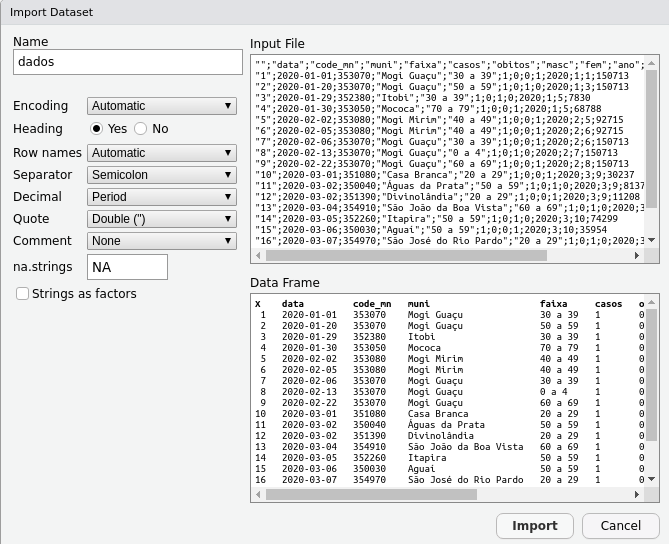
\includegraphics{ilustracoes/import_dataset.png}

\begin{center}\rule{0.5\linewidth}{0.5pt}\end{center}

\begin{center}\rule{0.5\linewidth}{0.5pt}\end{center}

\hypertarget{escrita-de-arquivos}{%
\section{Escrita de arquivos}\label{escrita-de-arquivos}}

\hypertarget{utilswrite.csv2}{%
\subsection{utils::write.csv2()}\label{utilswrite.csv2}}

Função para salvar um arquivo de dados que foi trabalhado no R em diferentes formatos, no caso, separado por ponto e vírgula. Um ponto negativo é que essa função, ao salvar o arquivo, cria uma coluna com nomes das linhas (em números).

\begin{quote}
\href{https://www.rdocumentation.org/packages/utils/versions/3.6.2/topics/write.table}{Documentação}
\end{quote}

\begin{quote}
\textbf{Exemplo}
\end{quote}

\begin{Shaded}
\begin{Highlighting}[]
\FunctionTok{write.csv2}\NormalTok{(}\AttributeTok{x =}\NormalTok{ iris,                }\CommentTok{\# Dados ativos}
           \AttributeTok{file =} \StringTok{\textquotesingle{}dados/iris.csv\textquotesingle{}}\NormalTok{, }\CommentTok{\# Caminho e nome do arquivo}
           \AttributeTok{fileEncoding =} \StringTok{"UTF{-}8"}\NormalTok{)  }\CommentTok{\# Encoding}

\FunctionTok{read.csv2}\NormalTok{(}\StringTok{\textquotesingle{}dados/iris.csv\textquotesingle{}}\NormalTok{, }\AttributeTok{nrows =} \DecValTok{4}\NormalTok{)}
\end{Highlighting}
\end{Shaded}

\begin{verbatim}
##   X Sepal.Length Sepal.Width Petal.Length Petal.Width Species
## 1 1          5.1         3.5          1.4         0.2  setosa
## 2 2          4.9         3.0          1.4         0.2  setosa
## 3 3          4.7         3.2          1.3         0.2  setosa
## 4 4          4.6         3.1          1.5         0.2  setosa
\end{verbatim}

\begin{quote}
\textbf{Argumentos principais}
\end{quote}

\begin{longtable}[]{@{}
  >{\raggedright\arraybackslash}p{(\columnwidth - 2\tabcolsep) * \real{0.5000}}
  >{\raggedright\arraybackslash}p{(\columnwidth - 2\tabcolsep) * \real{0.5000}}@{}}
\toprule()
\begin{minipage}[b]{\linewidth}\raggedright
Argumento
\end{minipage} & \begin{minipage}[b]{\linewidth}\raggedright
Definição
\end{minipage} \\
\midrule()
\endhead
x & Objeto a ser escrito, prefereincialmente uma matriz ou data.frame. \\
file & Nome do arquivo criado (pode conter o caminho) utilizando aspas '' ``. \\
append & Logical. Se TRUE os dados serão adicionados à última linha de um arquivo já existente, que deve ter o nome descrito em file, se FALSE qualquer arquivo com o nome descrito será sobrescrito. \\
na & String usada para valores ausentes nos dados. \\
dec & String para definir divisor de decimal, ex. dec = ``.''. \\
col.names & Logical. Indica se os nomes das colunas de x devem ser escritos junto com x, ou um vetor de caracteres dos nomes das colunas a serem escritos. \\
row.names & Logical. Cria coluna com nomes para linhas. \\
fileEncoding & String. Declara a codificação a ser usada para que possam ser recodificados à medida que são gravados. \\
\bottomrule()
\end{longtable}

\begin{center}\rule{0.5\linewidth}{0.5pt}\end{center}

\begin{center}\rule{0.5\linewidth}{0.5pt}\end{center}

\hypertarget{readrwrite_csv2}{%
\subsection{readr::write\_csv2()}\label{readrwrite_csv2}}

É semelhante à função anterior, mas executa a tarefa mais rápido, com a vantagem de não criar uma coluna com nomes das linhas.

\begin{quote}
\href{https://www.rdocumentation.org/packages/readr/versions/1.3.1/topics/write_delim}{Documentação}
\end{quote}

\begin{quote}
\textbf{Exemplo}
\end{quote}

\begin{Shaded}
\begin{Highlighting}[]
\NormalTok{readr}\SpecialCharTok{::}\FunctionTok{write\_csv2}\NormalTok{(}\AttributeTok{x =}\NormalTok{ iris, }\AttributeTok{file =} \StringTok{\textquotesingle{}dados/iris.csv\textquotesingle{}}\NormalTok{)}
\FunctionTok{read.csv2}\NormalTok{(}\AttributeTok{file =} \StringTok{\textquotesingle{}dados/iris.csv\textquotesingle{}}\NormalTok{, }\AttributeTok{nrows =} \DecValTok{2}\NormalTok{)}
\end{Highlighting}
\end{Shaded}

\begin{verbatim}
##   Sepal.Length Sepal.Width Petal.Length Petal.Width Species
## 1          5.1         3.5          1.4         0.2  setosa
## 2          4.9         3.0          1.4         0.2  setosa
\end{verbatim}

\begin{quote}
\textbf{Argumentos principais}
\end{quote}

\begin{longtable}[]{@{}
  >{\raggedright\arraybackslash}p{(\columnwidth - 2\tabcolsep) * \real{0.5000}}
  >{\raggedright\arraybackslash}p{(\columnwidth - 2\tabcolsep) * \real{0.5000}}@{}}
\toprule()
\begin{minipage}[b]{\linewidth}\raggedright
Argumento
\end{minipage} & \begin{minipage}[b]{\linewidth}\raggedright
Definição
\end{minipage} \\
\midrule()
\endhead
x & Um data frame ou tibble a ser escrito. \\
file & Caminho, nome do arquivo e extensão. \\
append & Se FALSE, irá sobrescrever um arquivo existente, caso exista. Se TRUE, será salvo a partir da última linha de um arquivo existente. \\
col\_names & Default TRUE. Primeira linha como nomes das colunas. Se FALSE, nomes das colunas não serão incluídos. \\
\bottomrule()
\end{longtable}

\begin{center}\rule{0.5\linewidth}{0.5pt}\end{center}

\begin{center}\rule{0.5\linewidth}{0.5pt}\end{center}

\hypertarget{writexlwrite_xlsx}{%
\subsection{writexl::write\_xlsx()}\label{writexlwrite_xlsx}}

Grava um dataframe em um arquivo xlsx. Para criar um xlsx com (várias) sheets nomeadas, basta definir x para uma lista nomeada de dataframe.

\begin{quote}
\href{https://www.rdocumentation.org/packages/writexl/versions/1.4.0/topics/write_xlsx}{Documentação}
\end{quote}

\begin{quote}
\textbf{Exemplo 1}
\end{quote}

\begin{Shaded}
\begin{Highlighting}[]
\NormalTok{writexl}\SpecialCharTok{::}\FunctionTok{write\_xlsx}\NormalTok{(}\AttributeTok{x =}\NormalTok{ iris,}
                    \AttributeTok{path =} \StringTok{\textquotesingle{}dados/iris.xlsx\textquotesingle{}}\NormalTok{,}
                    \AttributeTok{col\_names =} \ConstantTok{TRUE}\NormalTok{,}
                    \AttributeTok{format\_headers =} \ConstantTok{TRUE}\NormalTok{)}
\NormalTok{readxl}\SpecialCharTok{::}\FunctionTok{read\_excel}\NormalTok{(}\StringTok{\textquotesingle{}dados/iris.xlsx\textquotesingle{}}\NormalTok{, }\AttributeTok{n\_max =} \DecValTok{2}\NormalTok{)}
\end{Highlighting}
\end{Shaded}

\begin{verbatim}
## # A tibble: 2 x 5
##   Sepal.Length Sepal.Width Petal.Length Petal.Width Species
##          <dbl>       <dbl>        <dbl>       <dbl> <chr>  
## 1          5.1         3.5          1.4         0.2 setosa 
## 2          4.9         3            1.4         0.2 setosa
\end{verbatim}

\begin{quote}
\textbf{Exemplo 2}
\end{quote}

\begin{Shaded}
\begin{Highlighting}[]
\NormalTok{writexl}\SpecialCharTok{::}\FunctionTok{write\_xlsx}\NormalTok{(}\AttributeTok{path =} \StringTok{"dados/conjuntodadosnativos.xlsx"}\NormalTok{,}
           \AttributeTok{x =} \FunctionTok{list}\NormalTok{(}\AttributeTok{sheet1=}\NormalTok{iris, }\AttributeTok{sheet2=}\NormalTok{cars, }\AttributeTok{sheet3=}\NormalTok{mtcars))}

\NormalTok{readxl}\SpecialCharTok{::}\FunctionTok{read\_excel}\NormalTok{(}\AttributeTok{path =} \StringTok{\textquotesingle{}dados/conjuntodadosnativos.xlsx\textquotesingle{}}\NormalTok{,}
                   \AttributeTok{sheet =} \DecValTok{3}\NormalTok{, }
                   \AttributeTok{n\_max =} \DecValTok{2}\NormalTok{)}
\end{Highlighting}
\end{Shaded}

\begin{verbatim}
## # A tibble: 2 x 11
##     mpg   cyl  disp    hp  drat    wt  qsec    vs    am  gear  carb
##   <dbl> <dbl> <dbl> <dbl> <dbl> <dbl> <dbl> <dbl> <dbl> <dbl> <dbl>
## 1    21     6   160   110   3.9  2.62  16.5     0     1     4     4
## 2    21     6   160   110   3.9  2.88  17.0     0     1     4     4
\end{verbatim}

\begin{quote}
\textbf{Argumentos principais}
\end{quote}

\begin{longtable}[]{@{}
  >{\raggedright\arraybackslash}p{(\columnwidth - 2\tabcolsep) * \real{0.5000}}
  >{\raggedright\arraybackslash}p{(\columnwidth - 2\tabcolsep) * \real{0.5000}}@{}}
\toprule()
\begin{minipage}[b]{\linewidth}\raggedright
Argumento
\end{minipage} & \begin{minipage}[b]{\linewidth}\raggedright
Definição
\end{minipage} \\
\midrule()
\endhead
x & Data frame ou lista de data frames que serão salvos em planilhas (sheets). \\
path & Nome do arquuivo criado. \\
col\_names & Se TRUE, primera linha traz os nomes das colunas. \\
format\_headers & Inserir nomes das colunas. \\
\bottomrule()
\end{longtable}

\begin{center}\rule{0.5\linewidth}{0.5pt}\end{center}

\begin{center}\rule{0.5\linewidth}{0.5pt}\end{center}

\hypertarget{data.tablefwrite}{%
\subsection{data.table::fwrite()}\label{data.tablefwrite}}

Função para escrever .csv muito mais rápido (por exemplo, 2 segundos versus 1 minuto) e flexível. Máquinas modernas têm mais de uma CPU, então fwrite as usa; em todos os sistemas operacionais, incluindo Linux, Mac e Windows. Output em csv, csv2, tab, etc.

\begin{quote}
\href{https://www.rdocumentation.org/packages/data.table/versions/1.14.2/topics/fwrite}{Documentação}
\end{quote}

\begin{quote}
\textbf{Exemplo}
\end{quote}

\begin{Shaded}
\begin{Highlighting}[]
\NormalTok{dados }\OtherTok{\textless{}{-}}\NormalTok{ data.table}\SpecialCharTok{::}\FunctionTok{fread}\NormalTok{(}\AttributeTok{file =} \StringTok{\textquotesingle{}dados/dados.csv\textquotesingle{}}\NormalTok{, }\AttributeTok{nrows =} \DecValTok{20}\NormalTok{)}
\NormalTok{data.table}\SpecialCharTok{::}\FunctionTok{fwrite}\NormalTok{(}\AttributeTok{x =}\NormalTok{ dados,                     }\CommentTok{\# Objeto a ser escrito}
                   \AttributeTok{file =} \StringTok{\textquotesingle{}dados/dados20max.csv\textquotesingle{}}\NormalTok{, }\CommentTok{\# Nome e caminho (arquivo ja exite)}
                   \AttributeTok{append =} \ConstantTok{TRUE}\NormalTok{,                 }\CommentTok{\# Salva na ultima linha do arquivo ja existente}
                   \AttributeTok{sep =} \StringTok{\textquotesingle{};\textquotesingle{}}\NormalTok{,                     }\CommentTok{\# Separados de colunas}
                   \AttributeTok{showProgress =} \ConstantTok{TRUE}\NormalTok{)           }\CommentTok{\# Mostrar progresso}
\end{Highlighting}
\end{Shaded}

\begin{quote}
\textbf{Argumentos principais}
\end{quote}

\begin{longtable}[]{@{}
  >{\raggedright\arraybackslash}p{(\columnwidth - 2\tabcolsep) * \real{0.5000}}
  >{\raggedright\arraybackslash}p{(\columnwidth - 2\tabcolsep) * \real{0.5000}}@{}}
\toprule()
\begin{minipage}[b]{\linewidth}\raggedright
Argumento
\end{minipage} & \begin{minipage}[b]{\linewidth}\raggedright
Definição
\end{minipage} \\
\midrule()
\endhead
x & Objeto a salvar. Deve estar como data.frame ou data.table. \\
file & Nome do arquivo. \\
append & Se TRUE , o arquivo é salvo em acrescimo à última linha de um arquivo existente, sem incluir os nomes das colunas. \\
sep & Separador de colunas. Default é ``,''. \\
na & Um string a ser usada para valores ausentes. O padrão é uma string em branco ``\,``. \\
dec & Separador de decimal, default é ``.''. \\
row.names & Nome das linhas. Usar somente se for data.frame, porque é incompatível com data.table.. \\
col.names & Primeira linha como nomes das colunas. \\
logical01 & Os valores lógicos devem ser escritos como 1 e 0 em vez de ``TRUE'' e ``FALSE''? \\
showProgress & Exibir um medidor de progresso no console. Ignorado quando file == ``\,``. \\
compress & Se compress = ``auto'' e se o arquivo termina em .gz, o formato de saída é gzipado csv. Se compress = ``none'', o formato de saída é sempre csv. Se compress = ``gzip'', o formato é csv compactado com gzip. A saída para o console nunca é compactada com gzip mesmo se compress = ``gzip''. Por padrão, compress = ``auto''. \\
\bottomrule()
\end{longtable}

\begin{center}\rule{0.5\linewidth}{0.5pt}\end{center}

\begin{center}\rule{0.5\linewidth}{0.5pt}\end{center}

\hypertarget{rioexport}{%
\subsection{rio::export()}\label{rioexport}}

Semelhante a outros comandos de escrita de arquivos, o rio::export() permite gravar um data frame nos formatos habituais de texto. Para exportar uma lista de arquivos, usar o rio::export\_list().

\begin{quote}
\href{https://www.rdocumentation.org/packages/rio/versions/0.5.29/topics/export}{Documentação}.
\end{quote}

\begin{quote}
\textbf{Exempĺo}
\end{quote}

\begin{Shaded}
\begin{Highlighting}[]
\NormalTok{rio}\SpecialCharTok{::}\FunctionTok{export}\NormalTok{(}\AttributeTok{x =}\NormalTok{ iris,                  }\CommentTok{\# Objeto que será exportado.}
            \AttributeTok{file =} \StringTok{\textquotesingle{}dados/iris.xlsx\textquotesingle{}}\NormalTok{)  }\CommentTok{\# Caminho, nome e extensão.}
\end{Highlighting}
\end{Shaded}

\begin{quote}
\textbf{Argumentos principais}
\end{quote}

\begin{longtable}[]{@{}
  >{\raggedright\arraybackslash}p{(\columnwidth - 2\tabcolsep) * \real{0.5000}}
  >{\raggedright\arraybackslash}p{(\columnwidth - 2\tabcolsep) * \real{0.5000}}@{}}
\toprule()
\begin{minipage}[b]{\linewidth}\raggedright
Argumento
\end{minipage} & \begin{minipage}[b]{\linewidth}\raggedright
Definição
\end{minipage} \\
\midrule()
\endhead
x & Matriz ou data frame a ser escrita. Exceções são que x pode ser uma lista de dados se o formato de arquivo de saída for uma pasta de Excel .xlsx. Para exportar uma lista de quadros de dados para vários arquivos, use export\_list em vez disso. \\
file & Nome do arquivo. Deve especificar file e/ou format. \\
format & Sequência de caracteres opcional contendo o formato de arquivo, que pode ser usado para substituir o formato inferido a partir de file ou, em vez de especificar file, um arquivo com o nome do símbolo de x e a extensão de arquivo especificada será criado. Os atalhos incluem: ``,'' ou ``;'' ou '' \\
\bottomrule()
\end{longtable}

\begin{center}\rule{0.5\linewidth}{0.5pt}\end{center}

\begin{center}\rule{0.5\linewidth}{0.5pt}\end{center}

\hypertarget{leitura-de-muxfaltiplos-arquivos}{%
\section{Leitura de múltiplos arquivos}\label{leitura-de-muxfaltiplos-arquivos}}

Particularmente tenho maior interesse na possibilidade de ler e agrupar diversos arquivos, assim, o enfoque desse tópico será sobre a leitura com merge.

\hypertarget{baselapply-e-basereduce}{%
\subsection{base::lapply() e base::Reduce}\label{baselapply-e-basereduce}}

A ideia aqui é fazer a leitura dos arquivos de interesse e juntá-los verticalmente compondo um dataframe final, assim, o método é\\
dividido em três partes:\\
1. Listar os arquivos de interesse presentes no diretório.
2. Fazer leitura múltipla utilizando a função base::lapply e base::read.csv2 (pode ser outra).
3. Juntar os dataframes com base::Reduce e base::rbind.dataframe.

\begin{quote}
\href{https://www.rdocumentation.org/packages/base/versions/3.6.2/topics/lapply}{Documentação base::lapply}\\
\href{https://www.rdocumentation.org/packages/purrr/versions/0.2.5/topics/reduce}{Documentação base::reduce()}
\end{quote}

\begin{quote}
\textbf{Exemplo 1}
\end{quote}

\begin{verbatim}
setwd('arquivos/')              # Define a pasta que contém os arquivos
lista <- base::list.files()     # Captura os arquivos na pasta e atribui à uma lista
arquivos <- base::lapply(X = lista,   # Lista com os arquivos a serem lidos
                         FUN = read.csv2)  # Função escolhida para ler
unidos <- base::Reduce(x = arquivos,       # Lista de dataframes
                       f = base::rbind.data.frame)  # Função para empilhar
setwd("~/Documentos/Estudos R/guia_de_bolso") # Volta para diretorio inicial
\end{verbatim}

O base::setwd() é mais importante neste caso por conta da atividade do base::lapply, que não tem um argumento path para definir espaço de trabalho, então tem que ser definido antes.\\
A lista ``arquivos'' também pode ser aplicada à função data.table::rbindlist(), que terá o mesmo efeito.

\begin{quote}
\textbf{Exemplo 2}
\end{quote}

Aqui a ideia é realizar a leitura, mas filtrando os arquivos somente com os dados de interesse, ao mesmo tempo, para isso, vamos usar a função base::function(). Os parâmetros serão passados para essa função e ela será aplicada ao lapply.

\begin{verbatim}
setwd('arquivos2/')

filtro.fun <- function(x){                      # Cria uma função
  data.table::fread(file = x) %>% 
    dplyr::select("Petal.Length",               # Manipulações
                  "Petal.Width", 
                  "Species") %>%
    dplyr::filter(Petal.Length > .5) %>%
    setNames(nm = c("compr","largura","especie"))
}

lista <- list.files()
arquivos <- lapply(X = lista, FUN = filtro.fun)

unidos <- data.table::rbindlist(l = arquivos)  # Mesmo efeito do Reduce

setwd("~/Documentos/Estudos R/guia_de_bolso") # Volta para diretório inicial
\end{verbatim}

\begin{quote}
\href{https://www.rdocumentation.org/packages/base/versions/3.6.2/topics/function}{Documentação}
\end{quote}

\begin{center}\rule{0.5\linewidth}{0.5pt}\end{center}

\begin{center}\rule{0.5\linewidth}{0.5pt}\end{center}

\hypertarget{basefor}{%
\subsection{base::for()}\label{basefor}}

A função \texttt{for} permite criar um loop de execução de determinada ação, no caso, o loop do exemplo realizará a leitura de vários arquivos que serão atribuidos à uma lista. Com a lista é possível empilhar em um único data frame.\\
\textgreater{} \href{https://www.rdocumentation.org/packages/base/versions/3.6.2/topics/Control}{Documentação}

\begin{quote}
\textbf{Exemplo}
\end{quote}

\begin{Shaded}
\begin{Highlighting}[]
\NormalTok{x }\OtherTok{\textless{}{-}} \DecValTok{1}         \CommentTok{\# Objeto contador}
\NormalTok{arquivos }\OtherTok{\textless{}{-}} \FunctionTok{list}\NormalTok{(}\FunctionTok{rep}\NormalTok{(}\ConstantTok{NA}\NormalTok{, }\DecValTok{3}\NormalTok{)) }\CommentTok{\# O objeto que vai receber a leitura individual dos arquivos, deve ser uma lista vazia}
\NormalTok{lista }\OtherTok{\textless{}{-}} \FunctionTok{list.files}\NormalTok{(}\StringTok{\textquotesingle{}arquivos2/\textquotesingle{}}\NormalTok{) }\CommentTok{\# Lista com os arquivos a serem lidos}

\ControlFlowTok{for}\NormalTok{ (i }\ControlFlowTok{in}\NormalTok{ lista) \{      }\CommentTok{\# Para cada elemento da lista, executar:}
\NormalTok{  arquivos[[x]] }\OtherTok{\textless{}{-}} \FunctionTok{read.csv2}\NormalTok{(}\AttributeTok{file =} \FunctionTok{file.path}\NormalTok{(}\StringTok{\textquotesingle{}arquivos2\textquotesingle{}}\NormalTok{,i)) }\SpecialCharTok{\%\textgreater{}\%}  \CommentTok{\# Cada elemento lido é adicionado a um espaço vazio da lista de arquivos}
    \FunctionTok{filter}\NormalTok{(Sepal.Length }\SpecialCharTok{\textgreater{}} \FloatTok{5.5}\NormalTok{)}
\NormalTok{  x }\OtherTok{\textless{}{-}}\NormalTok{ x }\SpecialCharTok{+} \DecValTok{1}  \CommentTok{\# O contador define em que posição o arquivo lido será adicionado à lista de arquivos}
\NormalTok{\}}

\NormalTok{data.table}\SpecialCharTok{::}\FunctionTok{rbindlist}\NormalTok{(}\AttributeTok{l =}\NormalTok{ arquivos)[}\DecValTok{1}\SpecialCharTok{:}\DecValTok{3}\NormalTok{,]}
\end{Highlighting}
\end{Shaded}

\begin{verbatim}
##    Sepal.Length Sepal.Width Petal.Length Petal.Width Species
## 1:          5.8           4          1.2         0.2  setosa
## 2:          5.7         4.4          1.5         0.4  setosa
## 3:          5.7         3.8          1.7         0.3  setosa
\end{verbatim}

\begin{center}\rule{0.5\linewidth}{0.5pt}\end{center}

\begin{center}\rule{0.5\linewidth}{0.5pt}\end{center}

\hypertarget{rioimport_list}{%
\subsection{rio::import\_list()}\label{rioimport_list}}

Importa um alista de data frames de um vetor de nomes ou arquivo multi-objeto (planilha Excel, arquivo .Rdata etc).

\begin{quote}
\href{https://www.rdocumentation.org/packages/rio/versions/0.5.29/topics/import_list}{Documentação}
\end{quote}

\begin{quote}
\textbf{Exemplo}
\end{quote}

\begin{verbatim}
setwd('arquivos/')
lista <- list.files()
unidos <- rio::import_list(file = lista, # Lista com nomes dos arquivos do diretório
                 rbind = TRUE,    # Empilhar. Se FALSE retorna uma lista com os data frames
                 header = TRUE)   # Nomes das colunas
setwd("~/Documentos/Estudos R/guia_de_bolso")
\end{verbatim}

\begin{center}\rule{0.5\linewidth}{0.5pt}\end{center}

\begin{center}\rule{0.5\linewidth}{0.5pt}\end{center}

\hypertarget{escrita-de-muxfaltiplos-arquivos}{%
\section{Escrita de múltiplos arquivos}\label{escrita-de-muxfaltiplos-arquivos}}

\hypertarget{rioexport_list}{%
\subsection{rio::export\_list()}\label{rioexport_list}}

Exporta uma lista de data frames. A extensão colocada no nome do arquivo já direciona o formato, porém, pode-se usar o argumento sep = ``;'' ou outro para definir o desejado. Os nomes dos arquivos salvos podem ser declarados por um vetor, ex. c(``iris1.csv'',``iris2.csv''), ou usar o recurso \texttt{\%s}, ex. \texttt{\%s.csv} é o mesmo que \texttt{nome\_do\_objeto.csv}.

\begin{quote}
\href{https://www.rdocumentation.org/packages/rio/versions/0.5.26/topics/export_list}{Documentação}
\end{quote}

\begin{quote}
\textbf{Exemplo}
\end{quote}

\begin{Shaded}
\begin{Highlighting}[]
\NormalTok{rio}\SpecialCharTok{::}\FunctionTok{export\_list}\NormalTok{(}\AttributeTok{x =} \FunctionTok{list}\NormalTok{(}\AttributeTok{iris1 =}\NormalTok{ iris[}\DecValTok{1}\SpecialCharTok{:}\DecValTok{30}\NormalTok{,],   }\CommentTok{\# Lista nomeada dos objetos a serem salvos}
                          \AttributeTok{iris2 =}\NormalTok{ iris[}\DecValTok{60}\SpecialCharTok{:}\DecValTok{80}\NormalTok{,],}
                          \AttributeTok{iris3 =}\NormalTok{ iris[}\DecValTok{50}\SpecialCharTok{:}\DecValTok{70}\NormalTok{,]),}
                 \AttributeTok{file =} \StringTok{\textquotesingle{}arquivos2/\%s.csv\textquotesingle{}}\NormalTok{,      }\CommentTok{\# Caminho. Nome do arquivo contido em \%s automaticamente}
                 \AttributeTok{sep=}\StringTok{";"}\NormalTok{)     }\CommentTok{\# Separador}
\end{Highlighting}
\end{Shaded}

\begin{center}\rule{0.5\linewidth}{0.5pt}\end{center}

\begin{center}\rule{0.5\linewidth}{0.5pt}\end{center}

\hypertarget{cross}{%
\chapter{Cross-references}\label{cross}}

Cross-references make it easier for your readers to find and link to elements in your book.

\hypertarget{chapters-and-sub-chapters}{%
\section{Chapters and sub-chapters}\label{chapters-and-sub-chapters}}

There are two steps to cross-reference any heading:

\begin{enumerate}
\def\labelenumi{\arabic{enumi}.}
\tightlist
\item
  Label the heading: \texttt{\#\ Hello\ world\ \{\#nice-label\}}.

  \begin{itemize}
  \tightlist
  \item
    Leave the label off if you like the automated heading generated based on your heading title: for example, \texttt{\#\ Hello\ world} = \texttt{\#\ Hello\ world\ \{\#hello-world\}}.
  \item
    To label an un-numbered heading, use: \texttt{\#\ Hello\ world\ \{-\#nice-label\}} or \texttt{\{\#\ Hello\ world\ .unnumbered\}}.
  \end{itemize}
\item
  Next, reference the labeled heading anywhere in the text using \texttt{\textbackslash{}@ref(nice-label)}; for example, please see Chapter \ref{cross}.

  \begin{itemize}
  \tightlist
  \item
    If you prefer text as the link instead of a numbered reference use: \protect\hyperlink{cross}{any text you want can go here}.
  \end{itemize}
\end{enumerate}

\hypertarget{captioned-figures-and-tables}{%
\section{Captioned figures and tables}\label{captioned-figures-and-tables}}

Figures and tables \emph{with captions} can also be cross-referenced from elsewhere in your book using \texttt{\textbackslash{}@ref(fig:chunk-label)} and \texttt{\textbackslash{}@ref(tab:chunk-label)}, respectively.

See Figure \ref{fig:nice-fig}.

\begin{Shaded}
\begin{Highlighting}[]
\FunctionTok{par}\NormalTok{(}\AttributeTok{mar =} \FunctionTok{c}\NormalTok{(}\DecValTok{4}\NormalTok{, }\DecValTok{4}\NormalTok{, .}\DecValTok{1}\NormalTok{, .}\DecValTok{1}\NormalTok{))}
\FunctionTok{plot}\NormalTok{(pressure, }\AttributeTok{type =} \StringTok{\textquotesingle{}b\textquotesingle{}}\NormalTok{, }\AttributeTok{pch =} \DecValTok{19}\NormalTok{)}
\end{Highlighting}
\end{Shaded}

\begin{figure}

{\centering 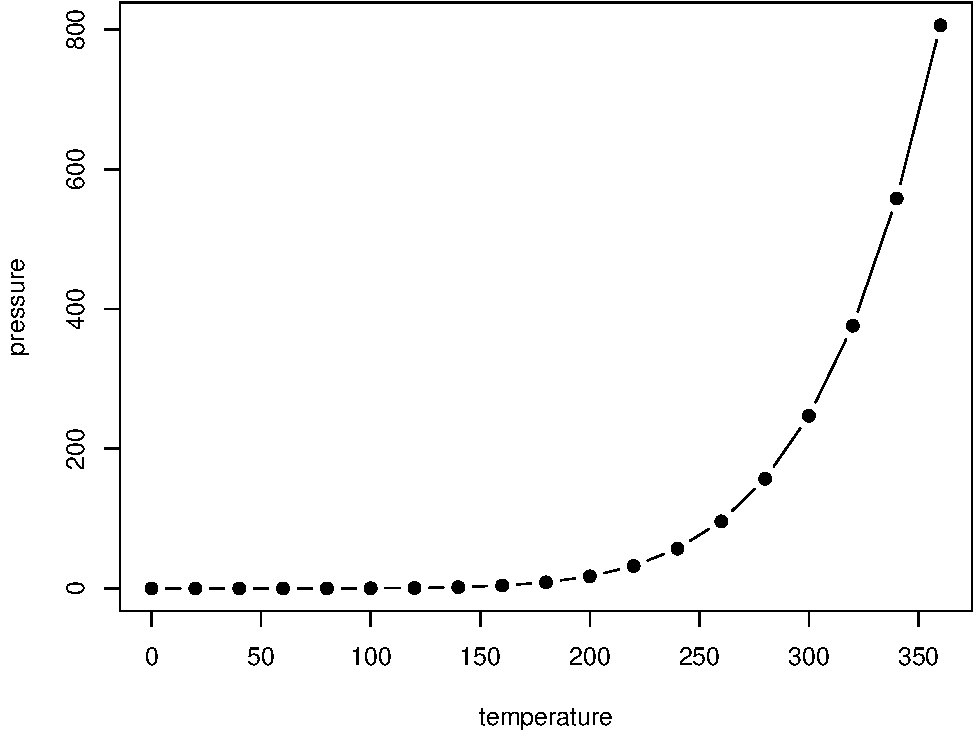
\includegraphics[width=0.8\linewidth]{guia_bolso_R_files/figure-latex/nice-fig-1} 

}

\caption{Here is a nice figure!}\label{fig:nice-fig}
\end{figure}

Don't miss Table \ref{tab:nice-tab}.

\begin{Shaded}
\begin{Highlighting}[]
\NormalTok{knitr}\SpecialCharTok{::}\FunctionTok{kable}\NormalTok{(}
  \FunctionTok{head}\NormalTok{(pressure, }\DecValTok{10}\NormalTok{), }\AttributeTok{caption =} \StringTok{\textquotesingle{}Here is a nice table!\textquotesingle{}}\NormalTok{,}
  \AttributeTok{booktabs =} \ConstantTok{TRUE}
\NormalTok{)}
\end{Highlighting}
\end{Shaded}

\begin{table}

\caption{\label{tab:nice-tab}Here is a nice table!}
\centering
\begin{tabular}[t]{rr}
\toprule
temperature & pressure\\
\midrule
0 & 0.0002\\
20 & 0.0012\\
40 & 0.0060\\
60 & 0.0300\\
80 & 0.0900\\
\addlinespace
100 & 0.2700\\
120 & 0.7500\\
140 & 1.8500\\
160 & 4.2000\\
180 & 8.8000\\
\bottomrule
\end{tabular}
\end{table}

\hypertarget{parts}{%
\chapter{Parts}\label{parts}}

You can add parts to organize one or more book chapters together. Parts can be inserted at the top of an .Rmd file, before the first-level chapter heading in that same file.

Add a numbered part: \texttt{\#\ (PART)\ Act\ one\ \{-\}} (followed by \texttt{\#\ A\ chapter})

Add an unnumbered part: \texttt{\#\ (PART\textbackslash{}*)\ Act\ one\ \{-\}} (followed by \texttt{\#\ A\ chapter})

Add an appendix as a special kind of un-numbered part: \texttt{\#\ (APPENDIX)\ Other\ stuff\ \{-\}} (followed by \texttt{\#\ A\ chapter}). Chapters in an appendix are prepended with letters instead of numbers.

\hypertarget{footnotes-and-citations}{%
\chapter{Footnotes and citations}\label{footnotes-and-citations}}

\hypertarget{footnotes}{%
\section{Footnotes}\label{footnotes}}

Footnotes are put inside the square brackets after a caret \texttt{\^{}{[}{]}}. Like this one \footnote{This is a footnote.}.

\hypertarget{citations}{%
\section{Citations}\label{citations}}

Reference items in your bibliography file(s) using \texttt{@key}.

For example, we are using the \textbf{bookdown} package \citep{R-bookdown} (check out the last code chunk in index.Rmd to see how this citation key was added) in this sample book, which was built on top of R Markdown and \textbf{knitr} \citep{xie2015} (this citation was added manually in an external file book.bib).
Note that the \texttt{.bib} files need to be listed in the index.Rmd with the YAML \texttt{bibliography} key.

The RStudio Visual Markdown Editor can also make it easier to insert citations: \url{https://rstudio.github.io/visual-markdown-editing/\#/citations}

\hypertarget{blocks}{%
\chapter{Blocks}\label{blocks}}

\hypertarget{equations}{%
\section{Equations}\label{equations}}

Here is an equation.

\begin{equation} 
  f\left(k\right) = \binom{n}{k} p^k\left(1-p\right)^{n-k}
  \label{eq:binom}
\end{equation}

You may refer to using \texttt{\textbackslash{}@ref(eq:binom)}, like see Equation \eqref{eq:binom}.

\hypertarget{theorems-and-proofs}{%
\section{Theorems and proofs}\label{theorems-and-proofs}}

Labeled theorems can be referenced in text using \texttt{\textbackslash{}@ref(thm:tri)}, for example, check out this smart theorem \ref{thm:tri}.

\begin{theorem}
\protect\hypertarget{thm:tri}{}\label{thm:tri}For a right triangle, if \(c\) denotes the \emph{length} of the hypotenuse
and \(a\) and \(b\) denote the lengths of the \textbf{other} two sides, we have
\[a^2 + b^2 = c^2\]
\end{theorem}

Read more here \url{https://bookdown.org/yihui/bookdown/markdown-extensions-by-bookdown.html}.

\hypertarget{callout-blocks}{%
\section{Callout blocks}\label{callout-blocks}}

The R Markdown Cookbook provides more help on how to use custom blocks to design your own callouts: \url{https://bookdown.org/yihui/rmarkdown-cookbook/custom-blocks.html}

\hypertarget{sharing-your-book}{%
\chapter{Sharing your book}\label{sharing-your-book}}

\hypertarget{publishing}{%
\section{Publishing}\label{publishing}}

HTML books can be published online, see: \url{https://bookdown.org/yihui/bookdown/publishing.html}

\hypertarget{pages}{%
\section{404 pages}\label{pages}}

By default, users will be directed to a 404 page if they try to access a webpage that cannot be found. If you'd like to customize your 404 page instead of using the default, you may add either a \texttt{\_404.Rmd} or \texttt{\_404.md} file to your project root and use code and/or Markdown syntax.

\hypertarget{metadata-for-sharing}{%
\section{Metadata for sharing}\label{metadata-for-sharing}}

Bookdown HTML books will provide HTML metadata for social sharing on platforms like Twitter, Facebook, and LinkedIn, using information you provide in the \texttt{index.Rmd} YAML. To setup, set the \texttt{url} for your book and the path to your \texttt{cover-image} file. Your book's \texttt{title} and \texttt{description} are also used.

This \texttt{gitbook} uses the same social sharing data across all chapters in your book- all links shared will look the same.

Specify your book's source repository on GitHub using the \texttt{edit} key under the configuration options in the \texttt{\_output.yml} file, which allows users to suggest an edit by linking to a chapter's source file.

Read more about the features of this output format here:

\url{https://pkgs.rstudio.com/bookdown/reference/gitbook.html}

Or use:

\begin{Shaded}
\begin{Highlighting}[]
\NormalTok{?bookdown}\SpecialCharTok{::}\NormalTok{gitbook}
\end{Highlighting}
\end{Shaded}


  \bibliography{book.bib,packages.bib}

\end{document}
